\documentclass[12pt]{article}
  
  \usepackage{article}
  
  \usepackage{graphicx,url}
  
  \usepackage[brazilian]{babel}
  \usepackage[utf8]{inputenc}
  \usepackage[T1]{fontenc}
  \usepackage{lipsum}
  
  
  \sloppy
  
  \title{Arquiteturas e modelos da computação em nuvem móvel: uma revisão sistemática}
  
  \author{Victor H. Fernandes\inst{1}, Marcelo M. Oliveira\inst{1}, Lucas M. \inst{1}}
  
  
  \address{Universidade de Brasília (UNB) - Campus FGA
  \\ Gama - DF - Brasil
  \email{\{victor.hmfd,martins.oliveira.mo,lucasamartins465\}@gmail.com}
  }
  
\begin{document} 

\maketitle

\begin{resumo} 
  A computação em nuvem móvel (MCC) é um conceito bastante novo, porém de grande impacto nas experiências de usabilidade
  dos usuários móveis, fornecendo a esses usuários, os serviços de processamento e armazenamento de dados nas nuvens.
  Os dispositivos móveis não precisam mais de uma configuração poderosa (por exemplo, velocidade da CPU e capacidade de memória)
  porque todos os módulos de computação complicados podem ser processados nas nuvem. Porém, por ser um conceito relativamento novo,
  ainda traz alguns desafios. Sendo assim, neste artigo, é apresentado uma revisão sistemática a cerca  das arquiteturas e modelos da
  computação em nuvem móvel, afim de investigar quais são os principais desafios da computação em nuvem em aplicativos móveis.
\end{resumo}

\begin{itemize}
 \item \textit{\textbf{Palavras-chave:} modelos de computação em nuvem em dispositivos movéis, Modelos MCC, modelos de nuvem em dispositivos
 movéis, arquitetura de nuvem em dispositivos movéis, computação em nuvem em dispositivos movéis, MCC, computação em dispositivos
 movéis, revisão da literatura na nuvem em dispositivos movéis, desafios de nuvem em dispositivos movéis, desafios.}
\end{itemize}

\begin{abstract}
  Mobile cloud computing (MCC) is a fairly new concept, but it has a major impact on the usability experiences 
  of mobile users, providing these users with the services of processing and storing data in the clouds. Mobile devices 
  no longer need a powerful configuration (for example, CPU speed and memory capacity) because all complicated computing 
  modules can be processed in the cloud. However, because it is a new concept, it still has some challenges. In this article, 
  a systematic review is presented about the architectures and models of mobile cloud computing, in order to investigate the 
  main challenges of cloud computing in mobile applications.
\end{abstract}

\begin{itemize}
 \item \textit{\textbf{Keywords:} mobile cloud computing models, MCC models, mobile cloud models, mobile cloud architecture, mobile cloud
 computing, MCC, mobile computing, mobile cloud literature review, mobile cloud challenges, challenges}
\end{itemize}




\section{Introdução}

\lipsum[1]

\section{Referencial Teórico}

Nesta seção é apresentado os conceitos da computação em nuvem e da computação em nuvem
móvel, bem como seus modelos e arquiteturas.

\subsection{Computação em Nuvem}

\subsection{Computação em Nuvem Móvel}

Aepona \cite{aepona2010} descreve a computação em nuvem móvel ou MCC(Mobile Cloud Computing) como um novo paradigma para aplicações 
móveis pelo qual o processamento e armazenamento de dados são movidos do dispositivo móvel para plataformas de computação
poderosas e centralizadas, localizadas em nuvens. Esses aplicativos são então acessados através da conexão sem fio com base em
um cliente ou navegador web nativo nos dispositivos móveis. 

Resumidamente, o MCC fornece aos usuários móveis os serviços de processamento e armazenamento de dados nas nuvens.
Os dispositivos móveis não precisam de uma configuração poderosa (por exemplo, velocidade da CPU e capacidade de memória)
porque todos os módulos de computação complicados podem ser processados nas nuvens \cite{liu2010}.

De acordo com Atta \cite{atta2013}, o principal objetivo da computação em nuvem é facilitar as pequenas empresas,
de forma econômica, fornecendo acesso a tecnologias que estão além do alcance deles. Ao usar a computação em nuvem, 
as pequenas empresas podem expandir seus recursos de TI com base em demandas de serviço e aproveitar oportunidades 
de crescimento para competir com outras empresas dentro do mercado.

Alternativamente, o principal objetivo da computação em nuvem móvel é fornecer experiências de usuários aprimoradas
aos usuários mobile que podem ser, em termos de tempo de computação, vida útil da bateria, comunicação, serviços e 
aprimoramento de recursos de dispositivos móveis.

Portanto, ambas as tecnologias têm objetivos e desafios diferentes. Por exemplo, na computação em nuvem móvel,
a conectividade de rede, a quantidade de comunicação, o custo de utilização da largura de banda e a energia do 
dispositivo móvel são considerados os principais problemas, o que pode não ser o caso na computação em nuvem.

No entanto, os modelos de aplicativos de nuvem móvel são baseados no modelo de serviço padrão da nuvem que inclui 
Infraestrutura como Serviço (IaaS), Plataforma como um serviço (PaaS) e Software as a Service (SaaS). Portanto, 
com base no funcionamento dos modelos de aplicativos, qualquer uma dessas camadas de serviço pode ser utilizada.
Alguns dos serviços bem conhecidos para computação em nuvem móvel incluem Amazon Elastic Compute Cloud (EC2) \cite{amazon}, 
Google App Engine \cite{googleapp} e Microsoft Azure \cite{azure}.

Atta \cite{atta2013} diz que não existe uma definição padrão ou caracterização de recursos da computação em nuvem móvel.
Portanto, apresenta uma comparação possível de computação em nuvem e computação em nuvem móvel, em termos de significância 
das questões listadas conforme tabela \ref{comparisonClouds}.

% ######## init table ########
\begin{table}[h]
  \centering
  % distancia entre a linha e o texto
  {\renewcommand\arraystretch{1.25}
  \begin{tabular}{ l l l }
    \cline{1-1}\cline{2-2}\cline{3-3}  
    \multicolumn{1}{|c|}{\textbf{Questões}} &
    \multicolumn{1}{c|}{\textbf{Computação em nuvem}} &
    \multicolumn{1}{c|}{\textbf{Computação em nuvem móvel}}
    \\  
    \cline{1-1}\cline{2-2}\cline{3-3}  
    \multicolumn{1}{|c|}{Energia do dispositivo} &
    \multicolumn{1}{c|}{x} &
    \multicolumn{1}{c|}{ok}
    \\  
    \cline{1-1}\cline{2-2}\cline{3-3}  
    \multicolumn{1}{|c|}{Custo de utilização da banda} &
    \multicolumn{1}{c|}{x} &
    \multicolumn{1}{c|}{ok}
    \\  
    \cline{1-1}\cline{2-2}\cline{3-3}  
    \multicolumn{1}{|c|}{Conectividade de rede} &
    \multicolumn{1}{c|}{x} &
    \multicolumn{1}{c|}{ok}
    \\  
    \cline{1-1}\cline{2-2}\cline{3-3}  
    \multicolumn{1}{|c|}{Mobilidade} &
    \multicolumn{1}{c|}{x} &
    \multicolumn{1}{c|}{ok}
    \\  
    \cline{1-1}\cline{2-2}\cline{3-3}  
    \multicolumn{1}{|c|}{Largura de Banda} &
    \multicolumn{1}{c|}{x} &
    \multicolumn{1}{c|}{ok}
    \\  
    \cline{1-1}\cline{2-2}\cline{3-3}  
    \multicolumn{1}{|c|}{Segurança} &
    \multicolumn{1}{c|}{ok} &
    \multicolumn{1}{c|}{ok}
    \\  
    \hline
    
  \end{tabular} }
  \caption{Comparação entre computação em nuvem e computação em nuvem móvel} 
  \label{comparisonClouds}
\end{table}


\subsubsection{Arquitetura da computação em nuvem móvel}


Na atual arquitetura de nuvem móvel, os dispositivos móveis podem acessar os serviços da nuvem de duas maneiras,
ou seja, através da rede móvel (rede de telecomunicações) ou através de pontos de acesso, conforme mostrado na Figura \ref{arquiteturaMCC}.

\begin{figure}[ht]
  \centering
  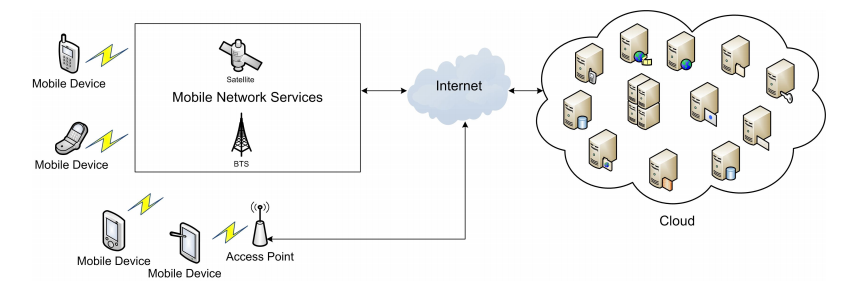
\includegraphics[scale= 0.5]{figuras/arquiteturaMCC.png}
  \caption{Arquitetura da computação em nuvem móvel}
  \label{arquiteturaMCC}
\end{figure}

No caso da rede móvel (provedor de rede de telecomunicações), os dispositivos móveis, como os celulares smartphones \cite{satelite},
estão conectados a uma rede móvel através de uma Estação Base (BS) ou através de um link de satélite. No entanto, 
se os smartphones não estiverem equipados com um módulo de comunicação por satélite, são utilizados dispositivos 
externos de comunicação por satélite \cite{spot}. As redes de telecomunicações estão mais conectadas à Internet e 
fornecem conectividade com a Internet aos usuários. Portanto, se os usuários tiverem conectividade de rede móvel, 
os usuários podem acessar serviços baseados em nuvem através da Internet.

No caso do ponto de acesso, os usuários móveis se conectam aos pontos de acesso através do Wi-Fi, que está mais conectado 
ao provedor de serviços de Internet para fornecer conectividade com a Internet aos usuários. Portanto, os usuários da nuvem móvel
podem acessar serviços baseados em nuvem sem utilizar serviços de telecomunicações, o que pode cobrar por tráfego de dados. 
Além disso, as conexões baseadas em Wi-Fi oferecem pouca latência e consomem menos energia em comparação com as conexões 3G \cite{cuervo2010}.
Conseqüentemente, usuários da nuvem móvel preferem usar conexões Wi-Fi sempre que acessíveis.

\section{Metodologia}

Para a elaboração deste estudo, foi realizada uma revisão sistemática de literatura,
ou SRL(Systematic Literature Review), de acordo com os critérios e o modelo adotado 
por \cite{kitchenham2012}. Para isso, a revisão foi divida em três fases: planejamento,
execução e análise dos resultados, onde cada fase será melhor detalhada nas subseções seguintes.
A fase de Análise dos resultados, por comtemplar a parte principal desse trabalho, será detalhada
na próxima seção.

\subsection{Planejamento}

A fase de planejamento foi dividida em etapas e estão detalhadas nos subtópicos a seguir:

\subsubsection{Questão de pesquisa}

Este estudo responde a seguinte questão de pesquisa:

\begin{itemize}
  \item QP: Quais os principais desafios da computação em nuvem em aplicativos móveis?
\end{itemize}

\subsubsection{Definição da string de busca}

Para obtenção de resultados relevantes a partir das pesquisas a serem realizadas, foi necessário a criação de uma string de busca.
Para a criação dessa string, foi utilizado o método PICO(Population, Intervention, Comparison, Output), que foi
proposto por \cite{SANTOS2007}. O método PICO é uma maneira de facilitar o entendimento da questão de pesquisa, transformando-a
em uma string de busca.

A tabela \ref{pico} mostra como o método PICO foi definido.


\begin{table}[h]
  \centering
  % distancia entre a linha e o texto
  {\renewcommand\arraystretch{1.25}
  \begin{tabular}{ l l }
    \cline{1-1}\cline{2-2}  
    \multicolumn{1}{|p{5cm}|}{Elemento PICO} &
    \multicolumn{1}{p{8cm}|}{Argumento}
    \\  
    \cline{1-1}\cline{2-2}  
    \multicolumn{1}{|p{5cm}|}{P (Population)} &
    \multicolumn{1}{p{8cm}|}{mobile cloud computing}
    \\  
    \cline{1-1}\cline{2-2}  
    \multicolumn{1}{|p{5cm}|}{I (Intervention)} &
    \multicolumn{1}{p{8cm}|}{mobile cloud computing models, mobile cloud models, mobile cloud architecture, MCC}
    \\  
    \cline{1-1}\cline{2-2}  
    \multicolumn{1}{|p{5cm}|}{C (Comparison)} &
    \multicolumn{1}{p{8cm}|}{não se aplica}
    \\  
    \cline{1-1}\cline{2-2}  
    \multicolumn{1}{|p{5cm}|}{O (Outcome)} &
    \multicolumn{1}{p{8cm}|}{mobile cloud literature review, mobile cloud challenges, challenges}
    \\  
    \hline
  \end{tabular} }
  \caption{Definição da string de busca utilizando o método PICO} 
  \label{pico} 
  
\end{table}

Com os principais argumentos que abordam a questão de pesquisa deste estudo, foi possível a confecção da string de busca,
para uma busca mais precisa sobre o tema. Abaixo segue a primeira string definida:

(“mobile cloud computing models” OR “MCC models”) AND ("Mobile cloud models") AND ("Mobile cloud architecture") AND (“Mobile
cloud computing” OR “MCC”)

Após um refinamento da string acima, foi elaborada outra string com mais argumentos, que nos possibilitou uma maior precisão
sobre o matérial encontrado
para a escrita desta SRL. Abaixo segue a segunda string definida:

(“mobile cloud computing models” OR “MCC models”) AND ("Mobile cloud models") AND ("Mobile cloud architecture") AND (“Mobile
cloud computing” OR “MCC”) AND (“mobile computing”) AND (“mobile cloud literature review”) AND (“mobile cloud challenges”) AND
(“challenges”)

\subsubsection{Bases de busca}

Com a string de busca montada, definiu-se as bases de busca que nos retornaram artigos para a escrita dessa SRL. As bases de 
dados utilizadas para as pesquisas foram as seguintes:

\begin{itemize}
  \item IEEE Xplore (http://ieeexplore.ieee.org/Xplore/home.jsp)
  \item ACM Digital Library (https://dl.acm.org/)
  \item SpringerLink (https://link.springer.com/)
  \item ScienceDirect(http://www.sciencedirect.com/)
\end{itemize}

\subsubsection{Critérios}

Para a escolha das publicações foram feitos dois tipos de critérios, critério de inclusão e critério de exclusão.
Esse critérios foram utilizados para que os artigos selecionados fossem relevantes para para compor este estudo.

Critérios de inclusão:

\begin{itemize}
  \item CI1: A publicação deve estar escrita em inglês ou português;
  \item CI2: A publicação deve ter sido publicada a partir de 2005;
  \item CI3: A publicação deve apresentar estudos relevantes ao tema proposto nesta revisão sistemática no abstract.
\end{itemize}

Após selecionar as publicações, foi utilizado o seguinte critério para a exclusão do restante das publicações:

\begin{itemize}
  \item CE1. O abstract da publicação foge do tema proposto.
\end{itemize}

\subsection{Execução}

Após a definição da string de busca, foi realizada a execução da busca nas bases citadas anteriormente. Realizada a primeira
busca, foram encontrados diversas publicações, utilizando os critérios de inclusão e exclusão para filtrar as publicações
encontradas, foi feita a extração dos principais dados para a realização dessa SRL. Realizando essa filtragem através dos
critérios de inclusão e exclusão, obtivemos a seguinte tabela \ref{publicações} com a quantidade de publicações relevantes
encontradas em cada base:


\begin{table}[h]
 \centering
% distancia entre a linha e o texto
 {\renewcommand\arraystretch{1.25}
 \begin{tabular}{ l l }
  \cline{1-1}\cline{2-2}  
    \multicolumn{1}{|p{4.500cm}|}{\textbf{Base pesquisada}} &
    \multicolumn{1}{p{4.500cm}|}{\textbf{Publicações encontradas}}
  \\  
  \cline{1-1}\cline{2-2}  
    \multicolumn{1}{|p{4.500cm}|}{\textbf{IEEE Xplore} \centering } &
    \multicolumn{1}{p{4.500cm}|}{7 \centering }
  \\  
  \cline{1-1}\cline{2-2}  
    \multicolumn{1}{|p{4.500cm}|}{\textbf{ACM Digital Library} \centering } &
    \multicolumn{1}{p{4.500cm}|}{4 \centering }
  \\  
  \cline{1-1}\cline{2-2}  
    \multicolumn{1}{|p{4.500cm}|}{\textbf{SpringerLink} \centering } &
    \multicolumn{1}{p{4.500cm}|}{2 \centering }
  \\  
  \cline{1-1}\cline{2-2}  
    \multicolumn{1}{|p{4.500cm}|}{\textbf{ScienceDirect} \centering } &
    \multicolumn{1}{p{4.500cm}|}{1 \centering }
  \\  
  \hline

 \end{tabular} }
 \caption{Publicações relevantes encontradas} 
 \label{publicações} 
\end{table}


%Exemplo para colocar figura

% \begin{figure}[ht]
  % \centering
  % \includegraphics[width=.5\textwidth]{fig1.jpg}
  % \caption{A typical figure}
  % \label{fig:exampleFig1}
% \end{figure}

\section{Análise dos Resultados}

Posteriormente a leitura das publicações, foi possível encontrar a resposta para a pergunta que guiou esta SRL.

QP: Quais os principais desafios da computação em nuvem em aplicativos móveis?

Foi possível constatar vários desafios enfrentados pela computação em nuvem em aplicativos móveis, estão listados abaixo os
principais desafios encontrados durante a análise das publicações:

\begin{itemize}
 \item Segundo \cite{kumar2014}, devido ao pouco armazenamento físico e a baixa quantidade de bateria que os dispositivos
 possuem, há uma tendência a recorrer ao “offloading computation”,que é a transferência do conteúdo do dispositivo para uma
 plataforma externa, contudo se torna necessário gastar mais tempo para lidar com segurança e confiabilidade, gerando assim um
 grande desafio;

  \item Segundo \cite{gao13} outros riscos da segurança dos dados na nuvem são:

    \begin{itemize}
      \item Os provedores são responsáveis pelos dados armazenados;
      \item Como os dados são armazenados, os problemas de privacidade deles fica na mão dos provedores de serviços;
      \item Caso o usuário queira mudar seu provedor de serviço, ele não saberá se todos os dados estarão completos, e se os
      dados que estavam armazenados com o provedor de serviço antigo, serão completamente apagados.
    \end{itemize}

 
 \item Outro desafio, é a segurança dos dados salvos em nuvem. Por mais que a tecnologia avance, terá uma grande dificuldade no
 quesito segurança, pois deve-se tomar cuidado não apenas com a segurança do aplicativo móvel, mas também no sistema de
 armazenamento em nuvem que se está usando, segundo \cite{kumar2014};
 
 \item A propriedade de dados, é um dos desafios da computação, segundo \cite{alizadeh2013}, uma pessoa pode comprar um serviço 
 de mídia(músicas, filmes e vídeos) disponível na nuvem e armazenar fisicamente em seu dispositivo, contudo pode vir a ocorrer da
 prestadora de serviços vir a falir e remover aquele conteúdo, fazendo com que a pessoa perca o serviço comprado;
 
 \item Para a utilização do serviço em nuvem é necessário ter acesso a rede. É necessário uma conexão estável e rápida com a
 Internet para que o usuário tenha acesso as informações salvas na nuvem \cite{alizadeh2013}.
 
\end{itemize}


\section{Considerações Finais}

\bibliographystyle{abbrv}
\bibliography{article}

\end{document}
